% Choose one to switch between slides and handout
\documentclass[]{beamer}
%\documentclass[handout]{beamer}

% Video Meta Data
\title{Smart Contracts and Decentralized Finance}
\subtitle{Development Workflow}
\author{Prof. Dr. Fabian Schär}
\institute{University of Basel}

% Config File
% Packages
\usepackage[utf8]{inputenc}
\usepackage{hyperref}
\usepackage{gitinfo2}
\usepackage{tikz}
 \usetikzlibrary{calc}
\usepackage{amsmath}
\usepackage{mathtools}
\usepackage{bibentry}
\usepackage{xcolor}
\usepackage{colortbl} % Add colour to LaTeX tables
\usepackage{caption}
\usepackage[export]{adjustbox}
\usepackage{pgfplots} \pgfplotsset{compat = 1.17}
\usepackage{makecell}
\usepackage{fancybox}
\usepackage{ragged2e}
\usepackage{fontawesome}
\usepackage{seqsplit}
\usepackage{tabularx}
\usepackage{tcolorbox}
\usepackage{booktabs} % use instead  \hline in tables

% Color Options
\definecolor{highlight}{rgb}{0.65,0.84,0.82}
\definecolor{focus}{rgb}{0.72, 0, 0}
\definecolor{lightred}{rgb}{0.8,0.5,0.5}
\definecolor{midgray}{RGB}{190,195,200}

 %UniBas Main Colors
\definecolor{mint}{RGB}{165,215,210}
\definecolor{anthracite}{RGB}{45,55,60}
\definecolor{red}{RGB}{210,5,55}

 %UniBas Color Palette (for graphics)
\definecolor{strongmint}{RGB}{30,165,165}
\definecolor{darkmint}{RGB}{0,110,110}
\definecolor{softanthracite}{RGB}{140,145,150}
\definecolor{brightanthracite}{RGB}{190,195,200}
\definecolor{softred}{RGB}{235,130,155}

%Custom Colors
\definecolor{lightergray}{RGB}{230, 230, 230}



% Beamer Template Options
\beamertemplatenavigationsymbolsempty
\setbeamertemplate{footline}[frame number]
\setbeamercolor{structure}{fg=black}
\setbeamercolor{footline}{fg=black}
\setbeamercolor{title}{fg=black}
\setbeamercolor{frametitle}{fg=black}
\setbeamercolor{item}{fg=black}
\setbeamercolor{}{fg=black}
\setbeamercolor{bibliography item}{fg=black}
\setbeamercolor*{bibliography entry title}{fg=black}
\setbeamercolor{alerted text}{fg=focus}
\setbeamertemplate{items}[square]
\setbeamertemplate{enumerate items}[default]
\captionsetup[figure]{labelfont={color=black},font={color=black}}
\captionsetup[table]{labelfont={color=black},font={color=black}}

\setbeamertemplate{bibliography item}{\insertbiblabel}

%tcolor boxes
\newtcolorbox{samplecode}[2][]{
  colback=mint, colframe=darkmint, coltitle=white,
  fontupper = \ttfamily\scriptsize, fonttitle= \bfseries\scriptsize,
  boxrule = 0mm, arc = 0mm,
  boxsep = 1.3mm, left = 0mm, right = 0mm, top = 0.5mm, bottom = 0mm, middle=0mm,
  #1,title=#2}
  
\newtcolorbox{keytakeaway}[2][]{
  colback=softred, colframe=red, coltitle=white,
  fontupper = \scriptsize, fonttitle= \bfseries\scriptsize,
  boxrule = 0mm, arc = 0mm,
  boxsep = 1.3mm, left = 0mm, right = 0mm, top = 0.5mm, bottom = 0mm, middle=0mm,
  #1,title=#2}

\newtcolorbox{exercise}[2][]{
  colback=brightanthracite, colframe=anthracite, coltitle=white,
  fontupper = \scriptsize, fonttitle= \bfseries\scriptsize,
  boxrule = 0mm, arc = 0mm,
  boxsep = 1.3mm, left = 0mm, right = 0mm, top = 0.5mm, bottom = 0mm, middle=0mm,
  #1,title=#2}



% Link Icon Command 
\newcommand{\link}{%
    \tikz[x=1.2ex, y=1.2ex, baseline=-0.05ex]{%
        \begin{scope}[x=1ex, y=1ex]
            \clip (-0.1,-0.1)
                --++ (-0, 1.2)
                --++ (0.6, 0)
                --++ (0, -0.6)
                --++ (0.6, 0)
                --++ (0, -1);
            \path[draw,
                line width = 0.5,
                rounded corners=0.5]
                (0,0) rectangle (1,1);
        \end{scope}
        \path[draw, line width = 0.5] (0.5, 0.5)
            -- (1, 1);
        \path[draw, line width = 0.5] (0.6, 1)
            -- (1, 1) -- (1, 0.6);
        }
    }

% Other commands
\newcommand\tab[1][0.5cm]{\hspace*{#1}} % for code boxes


% Read Git Data from Github Actions Workflow
% Defaults to gitinfo2 for local builds
\IfFileExists{gitInfo.txt}
	{\input{gitInfo.txt}}
	{
		\newcommand{\gitRelease}{(Local Release)}
		\newcommand{\gitSHA}{\gitHash}
		\newcommand{\gitDate}{\gitAuthorIsoDate}
	}

% Custom Titlepage
\defbeamertemplate*{title page}{customized}[1][]
{
  \vspace{-0cm}\hfill\includegraphics[width=2.5cm]{../config/logo_cif}
  \includegraphics[width=1.9cm]{../config/seal_wwz}
  \\ \vspace{2em}
  \usebeamerfont{title}\textbf{\inserttitle}\par
  \usebeamerfont{title}\usebeamercolor[fg]{title}\insertsubtitle\par  \vspace{1.5em}
  \small\usebeamerfont{author}\insertauthor\par
  \usebeamerfont{author}\insertinstitute\par \vspace{2em}
  \usebeamercolor[fg]{titlegraphic}\inserttitlegraphic
    \tiny \noindent \texttt{Release Ver.: \gitRelease}\\ 
    \texttt{Version Hash: \gitSHA}\\
    \texttt{Version Date: \gitDate}\\ \vspace{1em}
    
    
    \iffalse
  \link \href{https://github.com/cifunibas/Bitcoin-Blockchain-Cryptoassets/blob/main/slides/intro.pdf}
  {Get most recent version}\\
  \link \href{https://github.com/cifunibas/Bitcoin-Blockchain-Cryptoassets/blob/main/slides/intro.pdf}
  {Watch video lecture}\\ 
  
  \fi
  
  \vspace{1em}
  License: \texttt{Creative Commons Attribution-NonCommercial-ShareAlike 4.0 International}\\\vspace{2em}
  \includegraphics[width = 1.2cm]{../config/license}
}


% tikzlibraries
\usetikzlibrary{decorations.pathreplacing}
\usetikzlibrary{decorations.markings}
\usetikzlibrary{positioning}
\usetikzlibrary{calc}
\captionsetup{font=footnotesize}

%%%%%%%%%%%%%%%%%%%%%%%%%%%%%%%%%%%%%%%%%%%%%%
%%%%%%%%%%%%%%%%%%%%%%%%%%%%%%%%%%%%%%%%%%%%%%
\begin{document}

\thispagestyle{empty}
\begin{frame}[noframenumbering]
	\titlepage
\end{frame}
%%%

%%%
\begin{frame}{The Workflow}
	\begin{figure}
		\begingroup
			\tikzset{every picture/.style={scale=0.8}}
			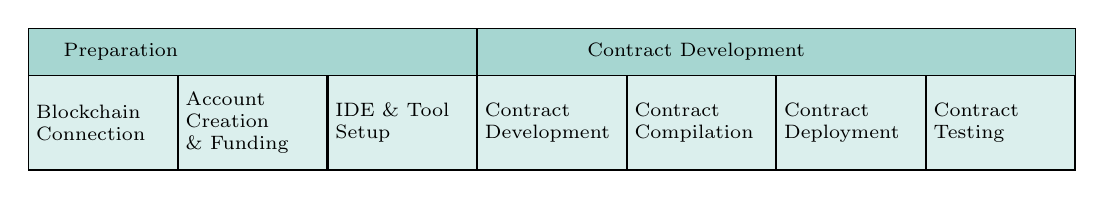
\begin{tikzpicture}[%
    node distance=1.9cm,
    on grid, every node/.append style={transform shape}
  ]
  
  \begin{scriptsize}
  
  \node[draw, rectangle, minimum height = 1.2cm, minimum width = 1.7cm, fill = highlight!40] (A)[text width = 1.7cm] at (0,0) {Blockchain\\ Connection};
  
  \node[draw, rectangle, minimum height = 1.2cm, minimum width = 1.7cm, fill = highlight!40] (B)[right of = A, text width = 1.7cm] {Account\\ Creation\\ \& Funding};
  
  \node[draw, rectangle, minimum height = 1.2cm, minimum width = 1.7cm, fill = highlight!40] (C)[right of = B, text width = 1.7cm] {IDE \& Tool\\ Setup};
  
  \node[draw, rectangle, minimum height = 0.6cm, minimum width = 5.7cm, fill = highlight] (B1)[text width = 4.8cm] at ($(A)!0.5!(C)+(0,0.9)$) {Preparation};
  
  \node[draw, rectangle, minimum height = 1.2cm, minimum width = 1.7cm, fill = highlight!40] (D)[right of = C, text width = 1.7cm] {Contract \\ Development};
  
  \node[draw, rectangle, minimum height = 1.2cm, minimum width = 1.7cm, fill = highlight!40] (E)[right of = D, text width = 1.7cm] {Contract \\ Compilation};
  
  \node[draw, rectangle, minimum height = 1.2cm, minimum width = 1.7cm, fill = highlight!40] (F)[right of = E, text width = 1.7cm] {Contract \\ Deployment};
  
  \node[draw, rectangle, minimum height = 1.2cm, minimum width = 1.7cm, fill = highlight!40] (G)[right of = F, text width = 1.7cm] {Contract \\ Testing};
  
  \node[draw, rectangle, minimum height = 0.6cm, minimum width = 7.6cm, fill = highlight] (G1)[text width = 4.8cm] at ($(D)!0.5!(G)+(0,0.9)$) {Contract Development};
  
  % \draw[->, transform canvas={yshift=-0.3cm}, color = highlight, ultra thick] (A.south west) -- (G.south east);
  
	\end{scriptsize}
	
\end{tikzpicture}
		\endgroup
	\end{figure}
	\vspace{1.5em}
\end{frame}
%%%

%%%
\begin{frame}{Blockchain Connection}

	\begin{figure}
		\begingroup
			\tikzset{every picture/.style={scale=0.6}}
			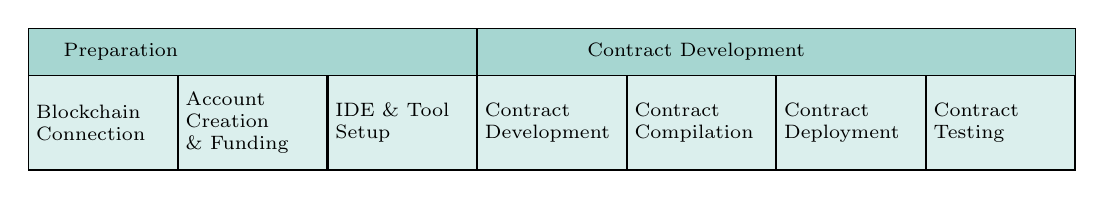
\begin{tikzpicture}[%
    node distance=1.9cm,
    on grid, every node/.append style={transform shape}
  ]
  
  \begin{scriptsize}
  
  \node[draw, rectangle, minimum height = 1.2cm, minimum width = 1.7cm, fill = highlight!40] (A)[text width = 1.7cm] at (0,0) {Blockchain\\ Connection};
  
  \node[draw, rectangle, minimum height = 1.2cm, minimum width = 1.7cm, fill = highlight!40] (B)[right of = A, text width = 1.7cm] {Account\\ Creation\\ \& Funding};
  
  \node[draw, rectangle, minimum height = 1.2cm, minimum width = 1.7cm, fill = highlight!40] (C)[right of = B, text width = 1.7cm] {IDE \& Tool\\ Setup};
  
  \node[draw, rectangle, minimum height = 0.6cm, minimum width = 5.7cm, fill = highlight] (B1)[text width = 4.8cm] at ($(A)!0.5!(C)+(0,0.9)$) {Preparation};
  
  \node[draw, rectangle, minimum height = 1.2cm, minimum width = 1.7cm, fill = highlight!40] (D)[right of = C, text width = 1.7cm] {Contract \\ Development};
  
  \node[draw, rectangle, minimum height = 1.2cm, minimum width = 1.7cm, fill = highlight!40] (E)[right of = D, text width = 1.7cm] {Contract \\ Compilation};
  
  \node[draw, rectangle, minimum height = 1.2cm, minimum width = 1.7cm, fill = highlight!40] (F)[right of = E, text width = 1.7cm] {Contract \\ Deployment};
  
  \node[draw, rectangle, minimum height = 1.2cm, minimum width = 1.7cm, fill = highlight!40] (G)[right of = F, text width = 1.7cm] {Contract \\ Testing};
  
  \node[draw, rectangle, minimum height = 0.6cm, minimum width = 7.6cm, fill = highlight] (G1)[text width = 4.8cm] at ($(D)!0.5!(G)+(0,0.9)$) {Contract Development};
  
  % \draw[->, transform canvas={yshift=-0.3cm}, color = highlight, ultra thick] (A.south west) -- (G.south east);
  
	\end{scriptsize}
	
\end{tikzpicture}
		\endgroup
	\end{figure}
		
	\textbf{What are you connecting to?}
	\begin{scriptsize}
	\uncover<2->{
	\begin{table}
		\centering
		\begin{tabular}{lllllll}
			
			
				\hline
				\rowcolor{highlight}
				\textbf{Network} & \textbf{Security} & \textbf{Speed} & \textbf{Access} & \textbf{Value} & \textbf{Cost} & \textbf{Ideal for} \\ \hline
			
				\begin{tabular}
					{@{}l@{}}Ethereum \\mainnet
				\end{tabular} & High & Slow & Public & Yes & ETH & Production \\
				\hline
			
			\uncover<3->{\href{https://ethereum.org/en/developers/docs/networks/\#testnets}{\begin{tabular}{@{}l@{}}\link Public \\ testnet \end{tabular}} & Low & Slow & Public & No & \begin{tabular}{@{}l@{}}Free \\ (Faucet) \end{tabular} & \begin{tabular}{@{}l@{}}Open \\ Alpha \end{tabular} \\ \hline}
			\uncover<4->{\begin{tabular}{@{}l@{}}Private \\ testnet \end{tabular} & Very low & Instant & Private & No & Free & \begin{tabular}{@{}l@{}}Early \\ Development \end{tabular} \\ \hline}
			\uncover<5->{\begin{tabular}{@{}l@{}}JavaScript \\ VM \end{tabular} & Very low & Instant & Private & No & Free & \\ \hline}
		\end{tabular}
		\label{tbl:mainnet_vs_testnet}
		\end{table}
	}
	\end{scriptsize}
	
	\uncover<6->{
	\small
	\textbf{How are you connecting?}	
	\vspace{-0.5em}
	\begin{columns}[T]
	\begin{column}{0.45\textwidth}
		\begin{itemize}
		\item \href{https://ethereum.org/en/developers/docs/nodes-and-clients/\#clients}{\link Local node}
		\begin{itemize}
			\item Best security
			\item Everything can be validated locally
		\end{itemize}
	\end{itemize}
	\end{column}
	\begin{column}{0.55\textwidth}
		\begin{itemize}
			\item<7-> Third party service (e.g., \href{https://infura.io/}{\link Infura} or \href{https://www.alchemy.com/}{\link Alchemy})
		\begin{itemize}
			\item<7-> Most convenient option
			\item<7-> But: heavily centralized
		\end{itemize}
	\end{itemize}
	\end{column}

	\end{columns}
	}
	
\end{frame}
%%%

%%%
\begin{frame}{Create Your Personal Chain with Ganache}

	\begin{columns}
		\begin{column}{0.15\textwidth}
			\begin{figure}
				\includegraphics[width = \textwidth]{../assets/images/logo_ganache.png}
			\end{figure}
		\end{column}
		\begin{column}{0.85\textwidth}
			\href{https://www.trufflesuite.com/ganache}{\link Ganache} quickly creates a private (Ethereum) Blockchain on your computer and prefunds 10 accounts with 100 custom Ether each. It is a great solution to quickly set up a private development chain.
		\end{column}
	\end{columns}
	\vspace{1.5em}
	\begin{exercise}{Exercise 4}
		\begin{enumerate}
			\item Install \href{https://www.trufflesuite.com/ganache}{\link Truffle Ganache} on your personal computer.
			\item Open Ganache and change hostname to local (0.0.0.0 -- all interfaces).
			\item Download \href{https://github.com/MyEtherWallet/etherwallet\#download-the-latest-release}{\link MyEtherWallet} and run it locally.
			\item Connect MyEtherWallet to your private chain. (https://localhost:8545)
			\item Import the Ganache mnemonic seed to MyEtherWallet.
			\item Make a transaction from account 1 to account 2.
		\end{enumerate}
	\end{exercise}
\end{frame}
%%%

%%%
\begin{frame}{Account Creation and Funding}

	\begin{figure}
		\begingroup
			\tikzset{every picture/.style={scale=0.6}}
			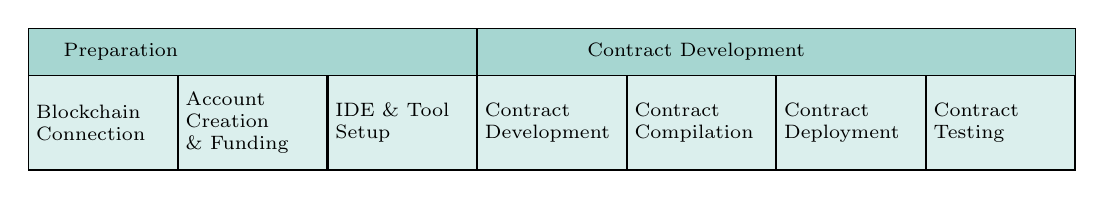
\begin{tikzpicture}[%
    node distance=1.9cm,
    on grid, every node/.append style={transform shape}
  ]
  
  \begin{scriptsize}
  
  \node[draw, rectangle, minimum height = 1.2cm, minimum width = 1.7cm, fill = highlight!40] (A)[text width = 1.7cm] at (0,0) {Blockchain\\ Connection};
  
  \node[draw, rectangle, minimum height = 1.2cm, minimum width = 1.7cm, fill = highlight!40] (B)[right of = A, text width = 1.7cm] {Account\\ Creation\\ \& Funding};
  
  \node[draw, rectangle, minimum height = 1.2cm, minimum width = 1.7cm, fill = highlight!40] (C)[right of = B, text width = 1.7cm] {IDE \& Tool\\ Setup};
  
  \node[draw, rectangle, minimum height = 0.6cm, minimum width = 5.7cm, fill = highlight] (B1)[text width = 4.8cm] at ($(A)!0.5!(C)+(0,0.9)$) {Preparation};
  
  \node[draw, rectangle, minimum height = 1.2cm, minimum width = 1.7cm, fill = highlight!40] (D)[right of = C, text width = 1.7cm] {Contract \\ Development};
  
  \node[draw, rectangle, minimum height = 1.2cm, minimum width = 1.7cm, fill = highlight!40] (E)[right of = D, text width = 1.7cm] {Contract \\ Compilation};
  
  \node[draw, rectangle, minimum height = 1.2cm, minimum width = 1.7cm, fill = highlight!40] (F)[right of = E, text width = 1.7cm] {Contract \\ Deployment};
  
  \node[draw, rectangle, minimum height = 1.2cm, minimum width = 1.7cm, fill = highlight!40] (G)[right of = F, text width = 1.7cm] {Contract \\ Testing};
  
  \node[draw, rectangle, minimum height = 0.6cm, minimum width = 7.6cm, fill = highlight] (G1)[text width = 4.8cm] at ($(D)!0.5!(G)+(0,0.9)$) {Contract Development};
  
  % \draw[->, transform canvas={yshift=-0.3cm}, color = highlight, ultra thick] (A.south west) -- (G.south east);
  
	\end{scriptsize}
	
\end{tikzpicture}
		\endgroup
	\end{figure}
	
	Depending on the blockchain you are working on, you get ETH in different ways:\\
	
	\begin{itemize}
		\item<1-> On \textbf{mainnet} you have to \textbf{buy Ether}	 (usually from an exchange).
		\item<2-> On \textbf{public testnets} you get Ether through an \textbf{Ether faucet}.
		\item<3-> On \textbf{private chains} you can simply \textbf{create new custom Ether}.
	\end{itemize}
	\vspace{1em}
	\uncover<4->{
	\begin{keytakeaway}{Additional Information on Private Chains}
		\href{https://souptacular.gitbooks.io/ethereum-tutorials-and-tips-by-hudson/content/private-chain.html}{\link Ethereum Tutorials and Tips by Hudson}
	\end{keytakeaway}
	}
\end{frame}
%%%

%%%
\begin{frame}{IDE and Tool Setup}

	\begin{figure}
		\begingroup
			\tikzset{every picture/.style={scale=0.6}}
			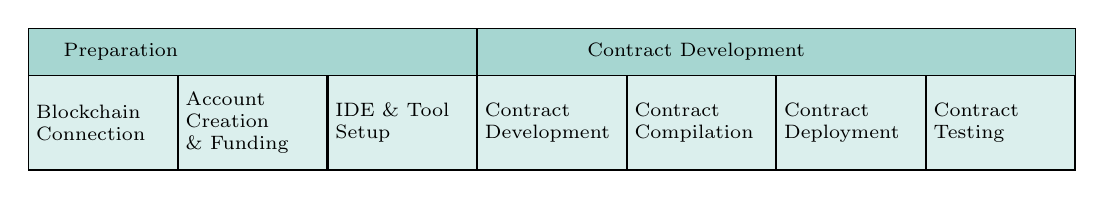
\begin{tikzpicture}[%
    node distance=1.9cm,
    on grid, every node/.append style={transform shape}
  ]
  
  \begin{scriptsize}
  
  \node[draw, rectangle, minimum height = 1.2cm, minimum width = 1.7cm, fill = highlight!40] (A)[text width = 1.7cm] at (0,0) {Blockchain\\ Connection};
  
  \node[draw, rectangle, minimum height = 1.2cm, minimum width = 1.7cm, fill = highlight!40] (B)[right of = A, text width = 1.7cm] {Account\\ Creation\\ \& Funding};
  
  \node[draw, rectangle, minimum height = 1.2cm, minimum width = 1.7cm, fill = highlight!40] (C)[right of = B, text width = 1.7cm] {IDE \& Tool\\ Setup};
  
  \node[draw, rectangle, minimum height = 0.6cm, minimum width = 5.7cm, fill = highlight] (B1)[text width = 4.8cm] at ($(A)!0.5!(C)+(0,0.9)$) {Preparation};
  
  \node[draw, rectangle, minimum height = 1.2cm, minimum width = 1.7cm, fill = highlight!40] (D)[right of = C, text width = 1.7cm] {Contract \\ Development};
  
  \node[draw, rectangle, minimum height = 1.2cm, minimum width = 1.7cm, fill = highlight!40] (E)[right of = D, text width = 1.7cm] {Contract \\ Compilation};
  
  \node[draw, rectangle, minimum height = 1.2cm, minimum width = 1.7cm, fill = highlight!40] (F)[right of = E, text width = 1.7cm] {Contract \\ Deployment};
  
  \node[draw, rectangle, minimum height = 1.2cm, minimum width = 1.7cm, fill = highlight!40] (G)[right of = F, text width = 1.7cm] {Contract \\ Testing};
  
  \node[draw, rectangle, minimum height = 0.6cm, minimum width = 7.6cm, fill = highlight] (G1)[text width = 4.8cm] at ($(D)!0.5!(G)+(0,0.9)$) {Contract Development};
  
  % \draw[->, transform canvas={yshift=-0.3cm}, color = highlight, ultra thick] (A.south west) -- (G.south east);
  
	\end{scriptsize}
	
\end{tikzpicture}
		\endgroup
	\end{figure}
		
	We recommend one of the following two IDEs:\\
	
	\begin{columns}
		\begin{column}{0.1\textwidth}
			\begin{figure}		\includegraphics[width = \textwidth]{../assets/images/logo_remix.png}
			\end{figure}
		\end{column}
		\begin{column}{0.85\textwidth}
			\textbf{\href{https://remix.ethereum.org/}{\link Remix}} is a browser-based IDE for solidity.\\
		\end{column}
	\end{columns}
	
	\begin{columns}
	\begin{column}{0.1\textwidth}
			\begin{figure}
				\includegraphics[width = \textwidth]{../assets/images/logo_atom.png}
			\end{figure}
		\end{column}
		\begin{column}{0.85\textwidth}
			\textbf{\href{https://atom.io/}{\link Atom}} is a general-purpose IDE. Make sure to download syntax highlighting packages for solidity.
		\end{column}
	\end{columns}
	
	\vspace{1em}
	
	\uncover<2->{
	For versioning purposes we recommend Git:\\
	
	\vspace{1em}
	
	\begin{columns}
	\begin{column}{0.1\textwidth}
			\begin{figure}
				\includegraphics[width = \textwidth]{../assets/images/logo_github.png}
			\end{figure}
		\end{column}
		\begin{column}{0.85\textwidth}
			\textbf{\href{https://github.com/}{\link GitHub}} is a hosting platform for Git repositories. Open Source projects are free and there is an educational account.
		\end{column}
	\end{columns}
	}
\end{frame}
%%%

%%%
\begin{frame}{Contract Development}
	\begin{figure}
		\begingroup
			\tikzset{every picture/.style={scale=0.6}}
			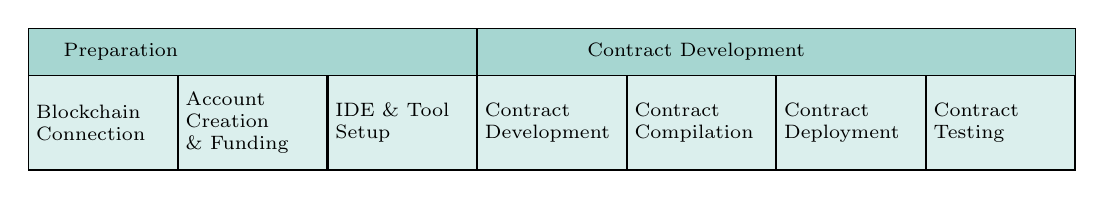
\begin{tikzpicture}[%
    node distance=1.9cm,
    on grid, every node/.append style={transform shape}
  ]
  
  \begin{scriptsize}
  
  \node[draw, rectangle, minimum height = 1.2cm, minimum width = 1.7cm, fill = highlight!40] (A)[text width = 1.7cm] at (0,0) {Blockchain\\ Connection};
  
  \node[draw, rectangle, minimum height = 1.2cm, minimum width = 1.7cm, fill = highlight!40] (B)[right of = A, text width = 1.7cm] {Account\\ Creation\\ \& Funding};
  
  \node[draw, rectangle, minimum height = 1.2cm, minimum width = 1.7cm, fill = highlight!40] (C)[right of = B, text width = 1.7cm] {IDE \& Tool\\ Setup};
  
  \node[draw, rectangle, minimum height = 0.6cm, minimum width = 5.7cm, fill = highlight] (B1)[text width = 4.8cm] at ($(A)!0.5!(C)+(0,0.9)$) {Preparation};
  
  \node[draw, rectangle, minimum height = 1.2cm, minimum width = 1.7cm, fill = highlight!40] (D)[right of = C, text width = 1.7cm] {Contract \\ Development};
  
  \node[draw, rectangle, minimum height = 1.2cm, minimum width = 1.7cm, fill = highlight!40] (E)[right of = D, text width = 1.7cm] {Contract \\ Compilation};
  
  \node[draw, rectangle, minimum height = 1.2cm, minimum width = 1.7cm, fill = highlight!40] (F)[right of = E, text width = 1.7cm] {Contract \\ Deployment};
  
  \node[draw, rectangle, minimum height = 1.2cm, minimum width = 1.7cm, fill = highlight!40] (G)[right of = F, text width = 1.7cm] {Contract \\ Testing};
  
  \node[draw, rectangle, minimum height = 0.6cm, minimum width = 7.6cm, fill = highlight] (G1)[text width = 4.8cm] at ($(D)!0.5!(G)+(0,0.9)$) {Contract Development};
  
  % \draw[->, transform canvas={yshift=-0.3cm}, color = highlight, ultra thick] (A.south west) -- (G.south east);
  
	\end{scriptsize}
	
\end{tikzpicture}
		\endgroup
	\end{figure}
		
	\begin{itemize}
		\item \textbf{Define your goal}
		\begin{itemize}
			\item What are you trying to achieve with your smart contract?
		\end{itemize}
		\item<2-> \textbf{Define your variables}
		\begin{itemize}
			\item<2-> What needs to be stored in the smart contract?
			\item<2-> Type and size needed.
		\end{itemize}
		\item<3-> \textbf{Define your functions}
		\begin{itemize}
			\item<3-> What is the function supposed to do?
			\item<3-> What are the input parameters?
			\item<3-> Are there any access restrictions?
		\end{itemize}
	\end{itemize}
\end{frame}
%%%

%%%
\begin{frame}{Storage Contract: Your First Smart Contract}
	
	\begin{columns}
		\begin{column}{0.15\textwidth}
			\begin{figure}
				\includegraphics[width = \textwidth]{../assets/images/box.png}
			\end{figure}
		\end{column}
		\begin{column}{0.85\textwidth}
			Remember the pseudo code example from earlier in this course?\\
			Let's create a \texttt{SharedStorage} contract where everyone can store an integer on the blockchain.
		\end{column}
	\end{columns}
	\vspace{1.5em}
	\begin{exercise}{Exercise 5}
		\begin{enumerate}
			\item Develop a contract with the two functions \texttt{\textcolor{focus}{store}(uint x)} and \texttt{\textcolor{focus}{read}()}.
			\item The function \texttt{\textcolor{focus}{store}(uint x)} is used to store an integer value in the contract. The function \texttt{\textcolor{focus}{read}()} allows anyone to lookup the value without the need for a transaction.
			\item Deploy the contract on your local Ganache testnet using the Remix Solidity IDE.
			\item Change the inital value to 133.
		\end{enumerate}
	\end{exercise}
\end{frame}
%%%

%%%
\begin{frame}{Storage Contract: Your First Smart Contract}
	\begin{samplecode}{Public Storage Contract:}
		pragma solidity \^{}0.7.0;\\
		\hfill
		
		contract SharedStorage \{ \\
		\hphantom{~~~~}uint dataStorage;\\
		\hfill
		
		\hphantom{~~~~}\textcolor{softanthracite}{// Set dataStorage value}\\
		\hphantom{~~~~}function \textcolor{focus}{store}(uint \_x) public \{ \\
			\hphantom{~~~~~~~~}dataStorage = \_x;\\
		\hphantom{~~~~}\} \\
		\hfill
		
		\hphantom{~~~~}\textcolor{softanthracite}{// Read dataStorage value}\\
		\hphantom{~~~~}function \textcolor{focus}{read}() public view returns (uint) \{ \\
			\hphantom{~~~~~~~~}return dataStorage;\\
			\hphantom{~~~~}\} \\
			\hfill
			
		\}
	\end{samplecode}
\end{frame}
%%%

%%%
\begin{frame}{Storage Contract: A More Compact Version}
	\begin{samplecode}{Public Storage Contract:}
		pragma solidity \^{}0.7.0;\\
		\hfill
		
		contract SharedStorage \{ \\
		\hphantom{~~~~}uint public dataStorage;\\
		\hfill
		
		\hphantom{~~~~}\textcolor{softanthracite}{// Set dataStorage value}\\
		\hphantom{~~~~}function \textcolor{focus}{store}(uint \_x) public \{ \\
			\hphantom{~~~~~~~~}dataStorage = \_x;\\
		\hphantom{~~~~}\} \\
		\hfill
		
		\}
	\end{samplecode}
	
	\begin{itemize}
		\item No explicit \texttt{\textcolor{focus}{read}()} function. Instead \texttt{public} function modifier.
		\item Getter function is automatically added.	
	\end{itemize}
\end{frame}
%%%


%%%
\begin{frame}{Contract Compilation}
	\begin{figure}
		\begingroup
			\tikzset{every picture/.style={scale=0.6}}
			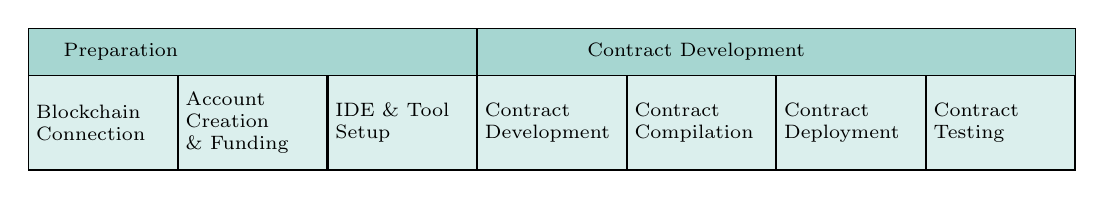
\begin{tikzpicture}[%
    node distance=1.9cm,
    on grid, every node/.append style={transform shape}
  ]
  
  \begin{scriptsize}
  
  \node[draw, rectangle, minimum height = 1.2cm, minimum width = 1.7cm, fill = highlight!40] (A)[text width = 1.7cm] at (0,0) {Blockchain\\ Connection};
  
  \node[draw, rectangle, minimum height = 1.2cm, minimum width = 1.7cm, fill = highlight!40] (B)[right of = A, text width = 1.7cm] {Account\\ Creation\\ \& Funding};
  
  \node[draw, rectangle, minimum height = 1.2cm, minimum width = 1.7cm, fill = highlight!40] (C)[right of = B, text width = 1.7cm] {IDE \& Tool\\ Setup};
  
  \node[draw, rectangle, minimum height = 0.6cm, minimum width = 5.7cm, fill = highlight] (B1)[text width = 4.8cm] at ($(A)!0.5!(C)+(0,0.9)$) {Preparation};
  
  \node[draw, rectangle, minimum height = 1.2cm, minimum width = 1.7cm, fill = highlight!40] (D)[right of = C, text width = 1.7cm] {Contract \\ Development};
  
  \node[draw, rectangle, minimum height = 1.2cm, minimum width = 1.7cm, fill = highlight!40] (E)[right of = D, text width = 1.7cm] {Contract \\ Compilation};
  
  \node[draw, rectangle, minimum height = 1.2cm, minimum width = 1.7cm, fill = highlight!40] (F)[right of = E, text width = 1.7cm] {Contract \\ Deployment};
  
  \node[draw, rectangle, minimum height = 1.2cm, minimum width = 1.7cm, fill = highlight!40] (G)[right of = F, text width = 1.7cm] {Contract \\ Testing};
  
  \node[draw, rectangle, minimum height = 0.6cm, minimum width = 7.6cm, fill = highlight] (G1)[text width = 4.8cm] at ($(D)!0.5!(G)+(0,0.9)$) {Contract Development};
  
  % \draw[->, transform canvas={yshift=-0.3cm}, color = highlight, ultra thick] (A.south west) -- (G.south east);
  
	\end{scriptsize}
	
\end{tikzpicture}
		\endgroup
	\end{figure}
		
	\textbf{The contract needs to be compiled to bytecode (and ABI).}\\
\end{frame}

\end{frame}
%%%

%%%
\begin{frame}{Contract Deployment}

	\begin{figure}
		\begingroup
			\tikzset{every picture/.style={scale=0.6}}
			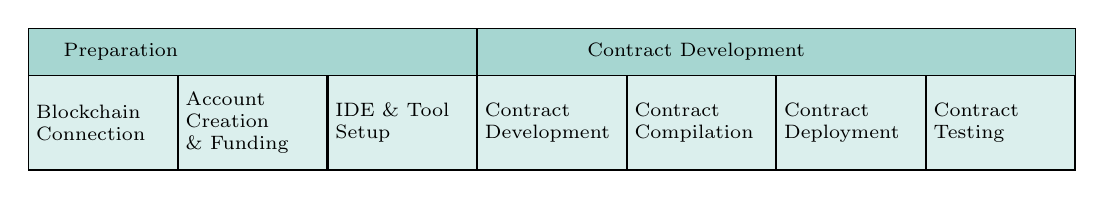
\begin{tikzpicture}[%
    node distance=1.9cm,
    on grid, every node/.append style={transform shape}
  ]
  
  \begin{scriptsize}
  
  \node[draw, rectangle, minimum height = 1.2cm, minimum width = 1.7cm, fill = highlight!40] (A)[text width = 1.7cm] at (0,0) {Blockchain\\ Connection};
  
  \node[draw, rectangle, minimum height = 1.2cm, minimum width = 1.7cm, fill = highlight!40] (B)[right of = A, text width = 1.7cm] {Account\\ Creation\\ \& Funding};
  
  \node[draw, rectangle, minimum height = 1.2cm, minimum width = 1.7cm, fill = highlight!40] (C)[right of = B, text width = 1.7cm] {IDE \& Tool\\ Setup};
  
  \node[draw, rectangle, minimum height = 0.6cm, minimum width = 5.7cm, fill = highlight] (B1)[text width = 4.8cm] at ($(A)!0.5!(C)+(0,0.9)$) {Preparation};
  
  \node[draw, rectangle, minimum height = 1.2cm, minimum width = 1.7cm, fill = highlight!40] (D)[right of = C, text width = 1.7cm] {Contract \\ Development};
  
  \node[draw, rectangle, minimum height = 1.2cm, minimum width = 1.7cm, fill = highlight!40] (E)[right of = D, text width = 1.7cm] {Contract \\ Compilation};
  
  \node[draw, rectangle, minimum height = 1.2cm, minimum width = 1.7cm, fill = highlight!40] (F)[right of = E, text width = 1.7cm] {Contract \\ Deployment};
  
  \node[draw, rectangle, minimum height = 1.2cm, minimum width = 1.7cm, fill = highlight!40] (G)[right of = F, text width = 1.7cm] {Contract \\ Testing};
  
  \node[draw, rectangle, minimum height = 0.6cm, minimum width = 7.6cm, fill = highlight] (G1)[text width = 4.8cm] at ($(D)!0.5!(G)+(0,0.9)$) {Contract Development};
  
  % \draw[->, transform canvas={yshift=-0.3cm}, color = highlight, ultra thick] (A.south west) -- (G.south east);
  
	\end{scriptsize}
	
\end{tikzpicture}
		\endgroup
	\end{figure}
		
	\begin{keytakeaway}{Contract Deployment}
		Creating your contract on the blockchain, i.e., sending a deployment transaction.
	\end{keytakeaway}
	
	\vspace{1.5em}
	\uncover<2->{
	\textbf{You can either \dots}
	\begin{itemize}
		\item<2-> \dots (compile and) deploy a contract directly from Remix.
		\item<3-> \dots use any wallet to migrate bytecode.
	\end{itemize}
	}
\end{frame}
%%%

%%%
\begin{frame}{Contract Testing}

	\begin{figure}
		\begingroup
			\tikzset{every picture/.style={scale=0.6}}
			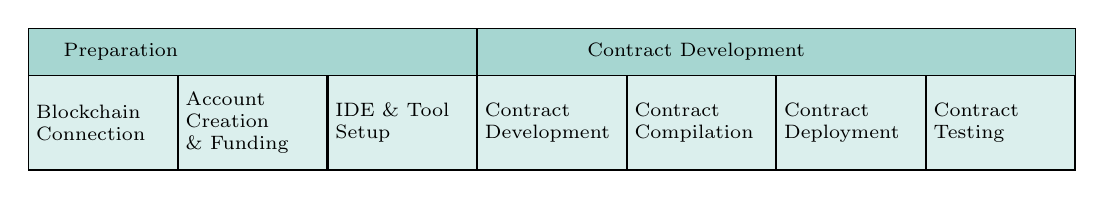
\begin{tikzpicture}[%
    node distance=1.9cm,
    on grid, every node/.append style={transform shape}
  ]
  
  \begin{scriptsize}
  
  \node[draw, rectangle, minimum height = 1.2cm, minimum width = 1.7cm, fill = highlight!40] (A)[text width = 1.7cm] at (0,0) {Blockchain\\ Connection};
  
  \node[draw, rectangle, minimum height = 1.2cm, minimum width = 1.7cm, fill = highlight!40] (B)[right of = A, text width = 1.7cm] {Account\\ Creation\\ \& Funding};
  
  \node[draw, rectangle, minimum height = 1.2cm, minimum width = 1.7cm, fill = highlight!40] (C)[right of = B, text width = 1.7cm] {IDE \& Tool\\ Setup};
  
  \node[draw, rectangle, minimum height = 0.6cm, minimum width = 5.7cm, fill = highlight] (B1)[text width = 4.8cm] at ($(A)!0.5!(C)+(0,0.9)$) {Preparation};
  
  \node[draw, rectangle, minimum height = 1.2cm, minimum width = 1.7cm, fill = highlight!40] (D)[right of = C, text width = 1.7cm] {Contract \\ Development};
  
  \node[draw, rectangle, minimum height = 1.2cm, minimum width = 1.7cm, fill = highlight!40] (E)[right of = D, text width = 1.7cm] {Contract \\ Compilation};
  
  \node[draw, rectangle, minimum height = 1.2cm, minimum width = 1.7cm, fill = highlight!40] (F)[right of = E, text width = 1.7cm] {Contract \\ Deployment};
  
  \node[draw, rectangle, minimum height = 1.2cm, minimum width = 1.7cm, fill = highlight!40] (G)[right of = F, text width = 1.7cm] {Contract \\ Testing};
  
  \node[draw, rectangle, minimum height = 0.6cm, minimum width = 7.6cm, fill = highlight] (G1)[text width = 4.8cm] at ($(D)!0.5!(G)+(0,0.9)$) {Contract Development};
  
  % \draw[->, transform canvas={yshift=-0.3cm}, color = highlight, ultra thick] (A.south west) -- (G.south east);
  
	\end{scriptsize}
	
\end{tikzpicture}
		\endgroup
	\end{figure}
		
	\textbf{Testing your contract is very important.}\\
	
	\begin{itemize}
		\item<2-> Manual testing
		\begin{itemize}
			\item<2-> Remix
			\item<2-> \href{}{\link Metamask}
			\item<2-> MyEtherWallet
		\end{itemize}
		\item<3-> Automated testing (e.g., Truffle and JavaScript test cases)
		\begin{itemize}
			\item<3-> Truffle (Automated JavaScript test cases)
		\end{itemize}
	\end{itemize}
\end{frame}
%%%

%%%
%\begin{frame}%[allowframebreaks]
%\frametitle{References and Recommended Reading}
%	\bibliographystyle{amsplain}
%	\bibliography{../assets/bib/refs}
%\end{frame}
%%%

\end{document}